\pdfoptionpdfminorversion=5
\documentclass{beamer}

\mode<presentation>
{
  \usetheme{Malmoe}
}

\usepackage{listings}
\usepackage[english]{babel}
\usepackage[latin1]{inputenc}
\usepackage{times}
\usepackage[T1]{fontenc}
\usepackage{eurosym}

\title[CF3 demo]{Coolfluid 3: Demonstration of current capabilities}

\date{16 Nov 2011}

\begin{document}

\section{Introduction}

\begin{frame}
 \frametitle{Coolfluid 3}
\begin{columns}
\begin{column}{5cm}
\begin{itemize}
 \item Started based on CF2 experience, as natural evolution
 \item Focus on flexibility and inter-operability between solvers
 \item Inter-institutional project
 \begin{itemize}
  \item IDIHOM
  \item PhD projects
  \item Institutions involved: VKI, VUB, RMA
 \end{itemize}
\item Open source
\end{itemize}
\end{column}
\begin{column}{5cm}
\begin{center}
 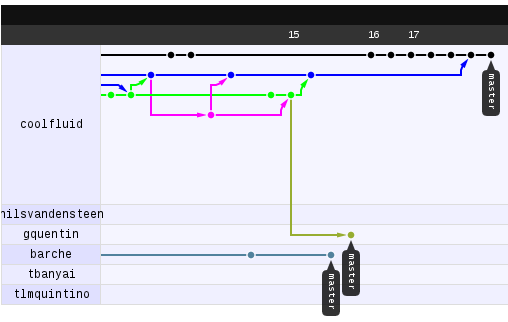
\includegraphics[width=5cm]{figs/github}\\
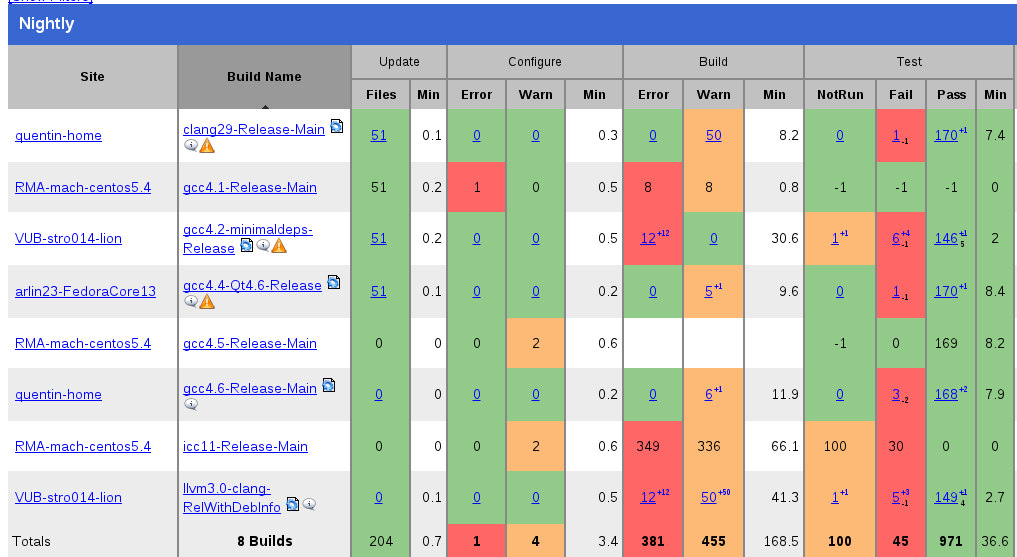
\includegraphics[width=5cm]{figs/dash}
\end{center}
\end{column}
\end{columns}
\end{frame}

\section{Component System}

\begin{frame}
 \frametitle{Component System}
\begin{itemize}
 \item Structure
 \begin{itemize}
  \item Tree of components, parents own children
  \item Access through ``file system'' path interface
 \end{itemize}
 \item Dynamic API
 \begin{itemize}
  \item Configuration using options
  \item Function calls through ``signals''
  \item Network-transparent
  \item Used for automatic UI and script binding interface
 \end{itemize}
 \item C++ API in the ``common'' library
\end{itemize}
\end{frame}

\section{GUI}

\begin{frame}
 \frametitle{GUI}
 \begin{itemize}
  \item Client-server system
  \item Server can control a parallel simulation on a cluster
  \item Mesh visualization using Paraview
  \item Dynamic generation, plugin authors don't need to do GUI programming
 \end{itemize}
\end{frame}

\section{Mesh}

\begin{frame}
 \frametitle{Mesh}
\end{frame}

\section{Conclusion}

\begin{frame}
 \frametitle{Current abilities}
\begin{itemize}
 \item Python scripting: 
  \begin{itemize}
   \item parametrization
   \item optimalization
   \item error analysis
  \end{itemize}
 \item Spectral difference
 \item Incompressible Finite Element solver
 \item Residual Distribution
 \item Proto language
 \item Parallelization
 \item LSS interface
\end{itemize}

\end{frame}


\end{document}
